\documentclass[10pt]{beamer}

\usetheme[subsectionpage=progressbar]{metropolis}
\usepackage{appendixnumberbeamer}

\usepackage{ucs}
\usepackage[utf8x]{inputenc}
\usepackage[ngerman]{babel}

\usepackage{booktabs}
\usepackage[scale=2]{ccicons}

\usepackage{pgfplots}
\usepgfplotslibrary{dateplot}

\usepackage{xspace}
\usepackage{dsfont}
\usepackage{graphicx}
\newcommand{\themename}{\textbf{\textsc{metropolis}}\xspace}

\title{Nummernschilderkennung mit Python}
% \subtitle{Machine Learning in Produktion und Logistik}
\date{19. Januar 2021}
\author{Anne-Sophie Bollmann, Susanne Kl\"ocker, Pia von Kolken, Christian Peters}
%\institute{TU Dortmund}
%\titlegraphic{\hfill\includegraphics[height=1.5cm]{logo.pdf}}

\begin{document}

\maketitle

\begin{frame}{Inhalt}
  \setbeamertemplate{section in toc}[sections numbered]
  \tableofcontents
\end{frame}

\section{Einleitung}

\begin{frame}{Einleitung}
    Hier kommt irgendwas fffff hin.
\end{frame}

\begin{frame}{Ein Titel}
    Hier kann man einfach was hinschreiben.
    Aufz\"ahlungen gehen nat\"urlich auch:
    \begin{itemize}
        \item Dies
        \item und
        \item das
    \end{itemize}
\end{frame}

\section{Objekterkennung}

\begin{frame}{Objekterkennung}
    Ein Beispiel f\"ur ein Zitat: Siehe \cite{hands_on}.
    \begin{itemize}
        \item Text in
        \item \textbf{fett}
        \item und
        \item \textit{kursiv}
    \end{itemize}
\end{frame}

\subsection{Deep Learning}

\begin{frame}{Ein Bild}
    \begin{figure}
        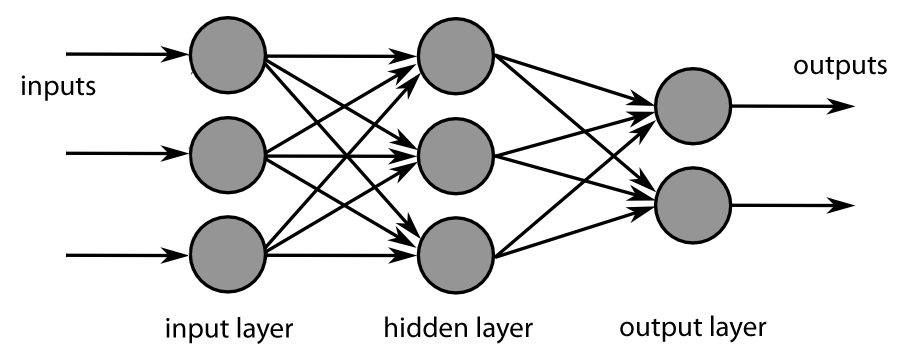
\includegraphics[height=0.5\textheight]{bilder/neuronales_netz.png}
        \caption{Ein neuronales Netz.}
    \end{figure}
\end{frame}

\section{Zeichenerkennung}

\begin{frame}{Zeichenerkennung}
    Beispiel Folie
\end{frame}

\begin{frame}[standout]
  Irgendwas zum Schluss
\end{frame}

\appendix

\begin{frame}[allowframebreaks]{Literatur}

  \bibliography{literatur}
  \bibliographystyle{abbrv}

\end{frame}

\end{document}
